% wave_spatial.tex
\documentclass[tikz,border=4pt]{standalone}
\usepackage{pgfplots}
\pgfplotsset{compat=1.18}
\renewcommand{\familydefault}{\sfdefault}

\begin{document}
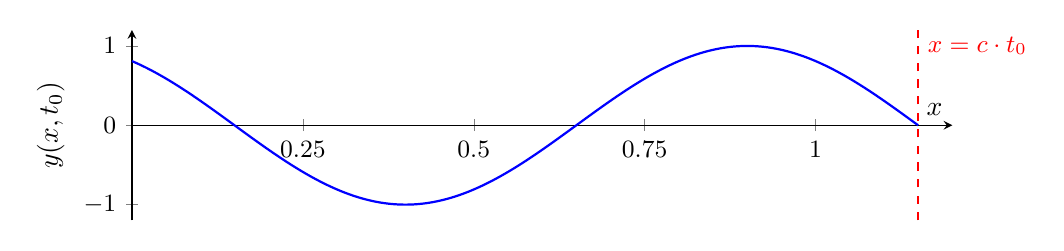
\begin{tikzpicture}
\pgfmathsetmacro{\A}{1}          % Amplitude
\pgfmathsetmacro{\lambda}{1}     % Wellenlänge
\pgfmathsetmacro{\k}{2*pi/\lambda}
\pgfmathsetmacro{\omega}{2*pi}   % Kreisfrequenz (f=1 Hz)
\pgfmathsetmacro{\tzero}{1.15}    % fester Zeitpunkt
\pgfmathsetmacro{\c}{\omega/\k}  % Wellengeschwindigkeit
\pgfmathsetmacro{\xfront}{\c*\tzero} % Wellenfront

\begin{axis}[
    width=12cm, height=4cm,
    xmin=0, xmax=1.2,
    ymin=-1.2, ymax=1.2,
    axis x line=middle, axis y line=left,
    xlabel={$x$}, ylabel={$y(x,t_0)$},
    xtick={0,0.25,0.5,0.75,1},
    ytick={-1,0,1},
    ticklabel style={font=\small},
    every axis plot/.append style={thick, blue},
    clip=false
]

% Welle bis zur Wellenfront
\addplot[samples=300,domain=0:\xfront] 
    {\A*sin(deg(\omega*\tzero - \k*x))};

% Wellenfront (vertikale gestrichelte Linie)
\addplot[domain=0:1,dashed,red] coordinates {(\xfront,-1.2) (\xfront,1.2)};
\node[anchor=west,font=\small, red] at (axis cs:\xfront,1) {$x=c \cdot t_0$};

\end{axis}
\end{tikzpicture}
\end{document}
